\documentclass[12pt,a4paper]{article}
\usepackage[utf8x]{inputenc}
\usepackage{ucs}
\usepackage[spanish]{babel}
\usepackage{amsmath}
\usepackage{amsfonts}
\usepackage{amssymb}
\usepackage{makeidx}
\usepackage{graphicx}
\usepackage[hidelinks]{hyperref}
\usepackage[left=2cm,right=2cm,top=2cm,bottom=2cm]{geometry}
\author{Reyes Alvarez Ulises Isaac\\4.B Ing. Mecatrónica\\Mtro. Carlos Enrique Morán Garabito\\Sistemas Electrónicos de Interfaz\\Sep - Dic 2019\\}
\title{Modulación de ancho de pulso}

\begin{document}
\maketitle
\begin{figure}[hbtp]
\centering

\includegraphics[scale=1.75]{Pictures/Universidad.png}
\end{figure}

\newpage
\section{¿Que es un PWM?}
Hablamos de la función PWM como abreviatura de la modulación por ancho de pulsos, algo que se ha convertido en una práctica habitual de los interruptores de potencia modernos, controlando la energía de inercia. Esta acción tiene en cuenta la modificación del proceso de trabajo de una señal de tipo periódico. Puede tener varios objetivos, como tener el control de la energía que se proporciona a una carga o llevar a cabo la transmisión de datos.
\begin{figure}[hbtp]
\centering
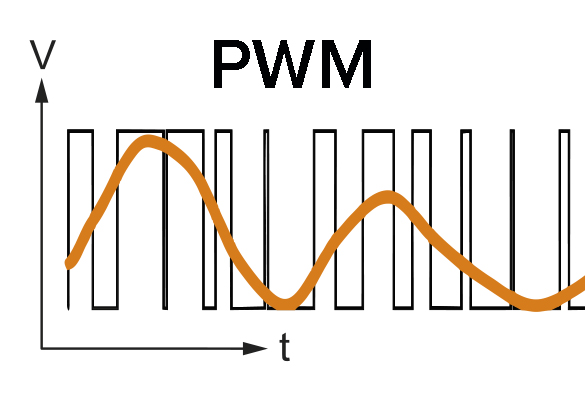
\includegraphics[scale=0.3]{Pictures/quees.jpg}
\caption{Señal de un PWM}
\end{figure}

\section{Para que sirve}
Tenemos que tener en cuenta distintos factores a la hora de hablar de los usos prácticos de la función PWM. Con el paso de los años y desde que la PWM entrara en vigor, las placas madre contaron con sensores de temperatura, consultables desde la bios del equipo. A partir de ese momento se impuso reducir el ruido de la CPU, haciendo que el ordenador reaccionara de distintas maneras en base al contexto. Si por ejemplo, estamos utilizando el equipo con el objetivo de descargar archivos, como demos de videojuegos, realmente el ordenador no necesita una potencia superior a la mínima. En estos casos la CPU no se calienta, no necesita el ventilador y se debe evitar gastar energía de forma innecesaria.\\

Cuando montamos un ordenador que deba poder ofrecer un rendimiento de primer nivel, pensamos en incluir la mayor potencia de ventilación, para que en situaciones críticas estos ventiladores puedan funcionar a toda máquina con el objetivo de evitar problemas en el equipo. Pero esta configuración se desaprovecha en momentos como en el ejemplo citado de la descarga de archivos. En estas situaciones no es necesario que el ventilador gire a toda velocidad, sino que se puede mantener en los niveles mínimos. La función PWM es una manera de regularlo. Para perfeccionar esto se le añadió un cable adicional que manda una señal de la velocidad a la que está funcionando el ventilador. La placa base se encarga de regular la velocidad a la que debe ir el ventilador en cada momento. Si el equipo se calienta mucho, le dice con una señal que debe trabajar más. Para ello hay que configurar el ordenador desde la bios siempre pensando en obtener los menores índices de ruido.Para que la función PWM tenga más sentido y sea más completa, existen accesorios que se encargan de llevar esa señal a otros ventiladores que también se puedan beneficiar de ella. El objetivo común es mejorar lo máximo posible el rendimiento de estos equipos.

\footnote{Universidad Politécnica de la Zona Metropolitana de Guadalajara}

\newpage
\section{Diseño del PWM}
Los amplificadores PWM  son dispositivos de conmutación de alto nivel cuyas tasas de elevación (slew rates) de voltaje y corriente, sobrepasan las encontradas en circuitos analógicos o digitales. Aunque el ancho de la banda de la señal no supere 1KHz, es muy útil adoptar el punto de vista del diseñador de Radio de Frecuencia; algunas cosas para tener en cuenta son: \\
* Inductancia del cable: 20 nH por pulgada\\
* Voltaje de una bobina: di / dt * L\\
* Corriente del condensador: dV / dT * C\\
* Una buena onda cuadrada: muy alto contenido armónicos\\

\section{Filtrado de la fuente}
Este aspecto del PWM es importante. El filtrado de la fuente es un trabajo que requiere de dos componentes para la correcta operación operación del amplificador. Utilice al menos 10mF por amperio de carga para filtrar las bajas frecuencias. Algunas aplicaciones necesitan mucha más capacitancia. Los condensadores con bajo ESR pueden facilitar el trabajo de encontrar espacio para grandes elementos.\\
Ubique este condensador a sólo algunos centímetros del amplificador. El filtro de alta frecuencia es muy delicado; piense en las frecuencias del rango entre 1 y 10 MHz. Recuerde que muchos condensadores parecen inductancias en este rango. Utilice capacitores cerámicos hasta completar 1mF o 10mF y conéctelos directamente entre los terminales de alimentación y tierra con el amplificador.\\
La función de los condensadores de filtro es poder satisfacer la demanda de corriente AC del amplificador, el cual está aislado de la fuente por la misma linea que lo conecta a ella. El grado de aislamiento se incrementa con la magnitud de la corriente, la frecuencia y la distancia. Cuando esté aislamiento impide el flujo de corriente desde la fuente, esta debe venir desde el condensador del filtrado.\\
Recuerde este requerimiento cuando selecciones los componentes los componentes y continúe con una medición de temperatura del prototipo o haga funcionar el sistema a máxima frecuencia y potencia hasta que la temperatura se estabilice. Durante este proceso recuerde que los capacitores que estén por debajo especificaciones pueden explotar.\\

\footnote{Universidad Politécnica de la Zona Metropolitana de Guadalajara}

\newpage
\section{Ciclo de trabajo}
Cuando la señal es alta (5V), la llamaremos “tiempo”. Para describir la cantidad de “tiempo”, se utiliza el concepto de ciclo de trabajo (duty cycle). El ciclo de trabajo se mide en porcentaje y describe específicamente el porcentaje de tiempo que una señal digital se encuentra en un estado alto en un intervalo o período de tiempo. Este período es el inverso de la frecuencia de la forma de onda. Si una señal digital pasa la mitad del tiempo encendido y la otra mitad apagada, diríamos que la señal digital tiene un ciclo de trabajo del 50\% por-ciento y se asemeja a una onda cuadrada ideal.\\
\begin{figure}[hbtp]
\centering
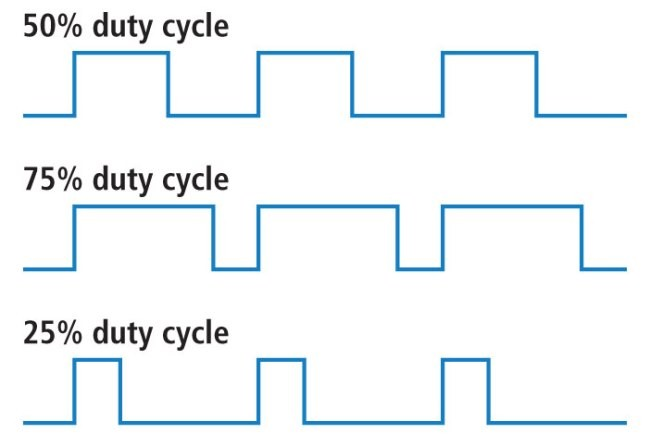
\includegraphics[scale=0.6]{Pictures/Ciclos.jpg}
\caption{Ejemplos de ciclos de trabajo}
\end{figure}
\footnote{Universidad Politécnica de la Zona Metropolitana de Guadalajara}

\newpage
\section{Etapa de acoplamiento}
La etapa de acoplamiento mostrada en la Figura 15, se usó para aislar la etapa de control de la etapa de potencia por medio de opto-acopladores. Los cuatro opto-acopladores, en este caso 6N135, portan la señal de conmutación para cada interruptor del puente inversor. Ya que cada señal es diferente para cada interruptor nos vemos en la necesidad de emplear
fuentes independientes de voltaje que provean de corriente y voltaje suficientes a la compuerta del interruptor para encenderlo. Así entonces, se usan 3 fuentes independientes de +15V, una para la activación de los interruptores de la parte superior del puente rectificador, y 2 para poder activar los interruptores de la parte inferior. Es importante notar que los
interruptores 1 y 3 comparten una fuente porque sus tierras coinciden en el mismo punto, por lo que se puede omitir el uso de una cuarta fuente. El primer transistor refuerza la señal de PWM para poder suministrar la corriente necesaria al diodo emisor del opto-acoplador. El último transistor es utilizado para invertir la señal del SPWM dada
por la configuración de transistor del opto-acoplador. Así, de este último transistor la señal de polarización del interruptor (voltaje compuerta (G) - emisor (E)) en el puente rectificador se toma de emisor y tierra.
\begin{figure}[hbtp]
\centering
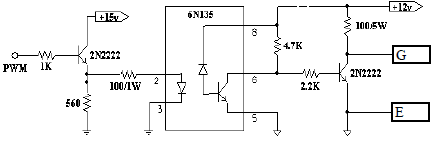
\includegraphics[scale=0.67]{Pictures/C.PNG}
\caption{Etapa de acoplamiento}
\end{figure}


\section{Circuito de potencia}
Ahora, a partir de una fuente de CA constante se debe
generar un voltaje de CD a partir de la conmutación de los 4 interruptores en el puente rectificador. Para ello se controlan 4 IGBTs de potencia ultrarrápidos(Qi=IRG4PC50U, VDSS=600V, ID=30A,) los cuales tienen la capacidad de conmutado rápido a parte de soportar rangos de voltajes altos. Además, se añadió una red snubber para los IGBTs con el objeto de protegerlos contra sobre tiros de tensión(R=100 Ohms y C=0.01mF). La alimentación de CA hacia el puente rectificador se reguló mediante un transformador variable y se tomaron mediciones de voltaje y corriente en el primario del transformador para medir el factor de potencia del convertidor.\\
\begin{figure}[hbtp]
\centering
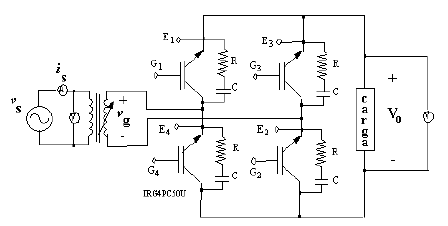
\includegraphics[scale=0.67]{Pictures/Circuito.PNG}
\caption{Circuito de Potencia}
\end{figure}

\footnote{Universidad Politécnica de la Zona Metropolitana de Guadalajara}

\newpage
\section{Generador de señales moduladas}
\begin{figure}[hbtp]
\centering
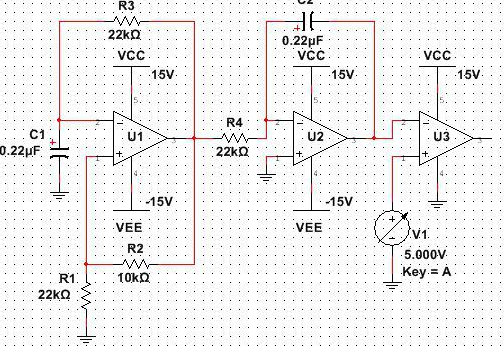
\includegraphics[scale=0.6]{Pictures/Generador.PNG}
\caption{Circuito generador de señales moduladas}
\end{figure}
\textbf{Formulas}
\begin{equation}
\frac{1}{T} = F = 1KHz\\
\end{equation}
\begin{equation}
T= \frac{1}{721Hz}= 1.387x10^-3 seg)\\
\end{equation}
\begin{equation}
T= 2 * R * C * Ln * (\frac{(1+B)}{(1-B)})
\end{equation}
\begin{equation}
B= \frac{R2}{R1+R2}
\end{equation}
\begin{equation}
B= \frac{500\Omega}{1k\Omega + 500\Omega}
\end{equation}
\begin{equation}
B= \frac{1}{3}
\end{equation}

\begin{figure}[hbtp]
\centering
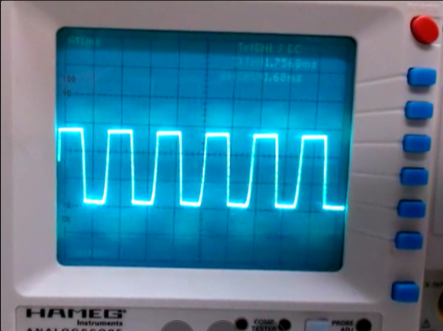
\includegraphics[scale=0.7]{Pictures/Onda.PNG}
\caption{Señal de la onda}
\end{figure}
\footnote{Universidad Politécnica de la Zona Metropolitana de Guadalajara}

\newpage
\section{Referencias Bibliográficas}
\url{https://www.ibertronica.es/blog/tutoriales/funcion-pwm/}\\

\url{https://revistas.udistrital.edu.com}\\

\url{https://cursos.mcielectronics.cl/2019/06/18/modulacion-por-ancho-de-pulsos/}\\


\footnote{Universidad Politécnica de la Zona Metropolitana de Guadalajara}

\end{document}